\documentclass{article}

\usepackage{amsmath}
\usepackage{graphicx}
\usepackage{hyperref}

\usepackage[margin=0.6in]{geometry}

\title{Optimization Algorithm's from AI course}
% \author{Filip Dabkowski}
\date{\today}

\begin{document}

\maketitle

\section{Objective}
Let's setup some objective to optimize as an example of usage. A common thing to optimize is fitting a line or more generally a function through some data.\newline

So first we need to get or generate some data. Like for example scores of students from Statistics exam, in relation to how much they like Statistics.
\begin{figure}[h]
    \centering
    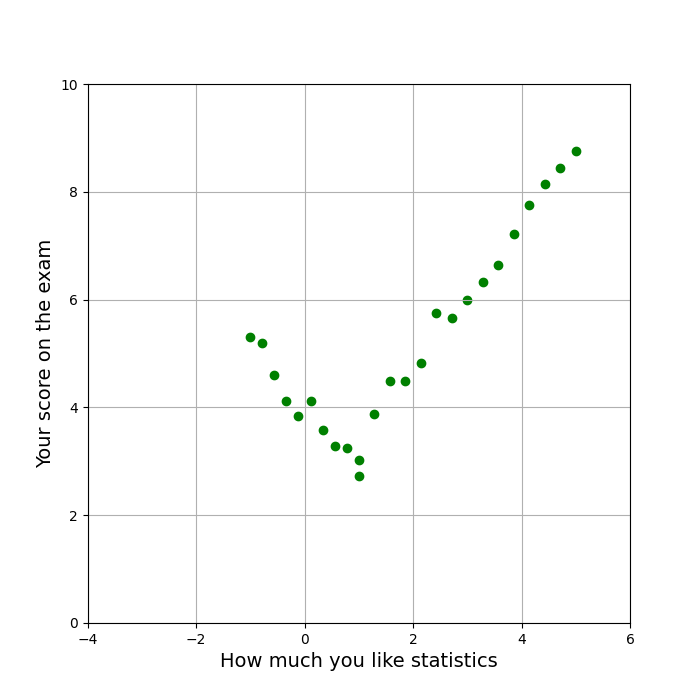
\includegraphics[width=0.4\textwidth]{../images/myplot1.png}
    \caption{Example data}
    \label{fig:data}
\end{figure}

Now that we have our data, we can denote $x$ as measure of likeness and $y$ as grade of the student. In that case each point on our graph is $(x_i, y_i)$, where $i$ is number of student in the dataset.

\break

Lets begin with defining our function that is going to approximate the data, it could also be used later for making predictions. Like ''If your likeness of Statistics equals 4, you will probably get 7.74 on your final exam''

\begin{figure}[h]
    \centering
    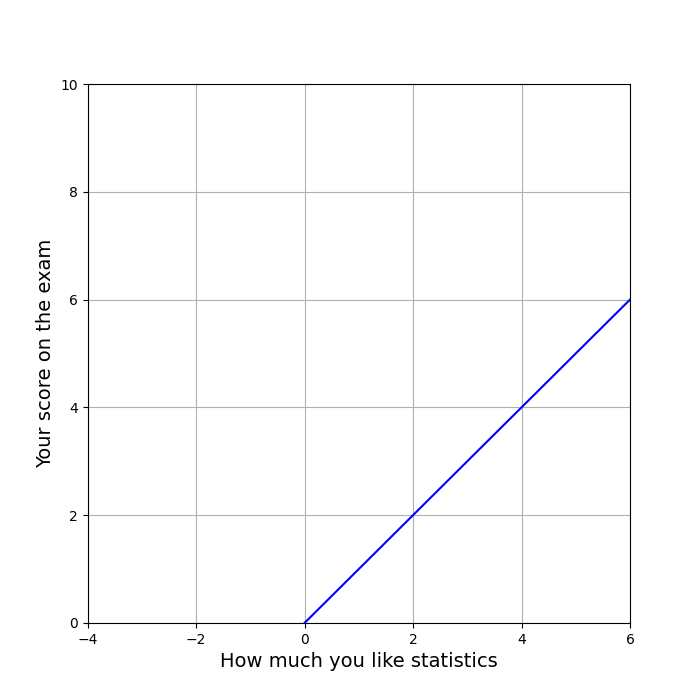
\includegraphics[width=0.4\textwidth]{../images/myplot2.png}
    \caption{Linear function $f(x) = 1 * x + 0$}
    \label{fig:data_line}
\end{figure}

Suppose our data can be approximated using a linear function, in our case it is not really true, however in real life we also can't visualize the whole dataset on a simple graph. Now we need some measure how well our model (function) fits the data (loss-function), so is it a good approximation or not. A common way to measure it, would be to calculate the squared difference between the actual value predicted value.

\begin{equation}
    \mathcal{L} = \sum_{i=1}^N{(y_i - f(x_i))^2}
\end{equation}

\textit{Side note, the loss function written above has a name (unfortunately more than one) Sum Squared Error (SSE), in ML circles it is more commonly know as L2 loss. It also has a more fancy notation, that you might find in papers... or YT videos.}

\begin{equation}
    L2 = || y - f(x) ||^2_2 = \sum_{i=1}^N{(y_i - f(x_i))^2}
\end{equation}

Now as you may see we have our loss-function that represent how badly our model preforms. If our loss were to reach 0 that would mean that the model perfectly fits the data. \textit{But how can we change our loss?} Of course by changing parameters in our model. The function $f(x) = 1 * x + 0$ has two parameters, currently set to $a=1$ and $b=0$, so our parametrized linear function is written as $f(x) = ax+b$. Now by changing parameters $a$ and $b$ we can lower or increase the loss. Now the expanded formula for the loss function is:

\begin{equation}
    \mathcal{L} = \sum_{i=1}^N{(y_i - (ax_i + b))^2}
\end{equation}

On the side note, the equation above is for the total loss, total since it is the sum of the loss of every point. More commonly used would be Mean Square Error (MSE) so basic average of the total loss.

\begin{equation}
    \mathcal{L} = \frac{1}{N}\sum_{i=1}^N{(y_i - (ax_i + b))^2}
\end{equation}

\section{Enumeration Method}
This is one of the simplest algorithms to understand, as the only thing that you need to do is to procedurally iterate through possible parameter values.\newline

The problem with that in our case is that possible values of the parameters $a$ and $b$ belong to real numbers. In math terms: $(a, b) \in \mathbf{R}\times\mathbf{R}$. So if we were to try plug in all the possible values for $a$ and $b$ we would be calculating forever with infinite precision. As a simplification we will only consider values in a range of $[-5,5]$ with step of $0.2$.

So now basically what we need to do is to alter both parameter's a little bit, changing our function and after each iteration of changing the parameter's, calculate the loss. We pick the pair of $a$ and $b$ parameter values that results in the smallest loss.

\begin{figure}[h]
    \centering
    \begin{minipage}{0.4\textwidth}
        \centering
        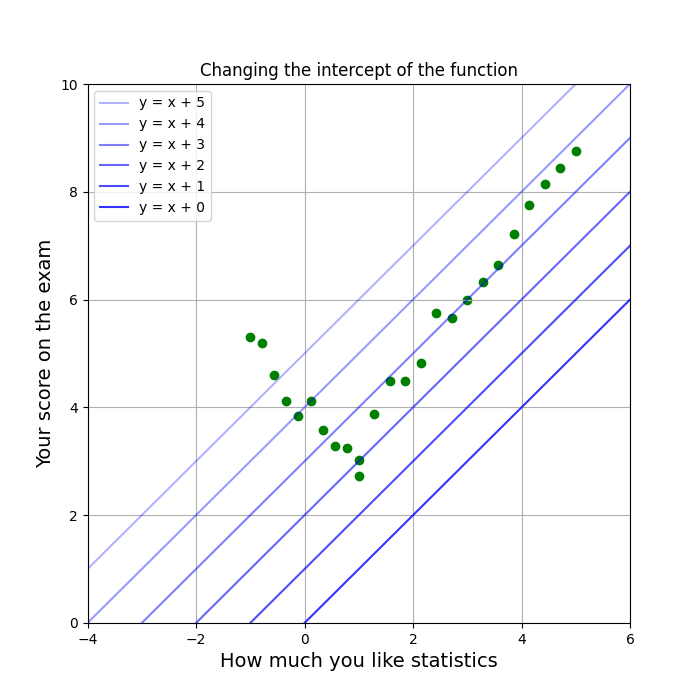
\includegraphics[width=\linewidth]{../images/myplot3.png}
        \caption{Altering the intercept parameter of our model}
    \end{minipage}
    \hfill
    \begin{minipage}{0.4\textwidth}
        \centering
        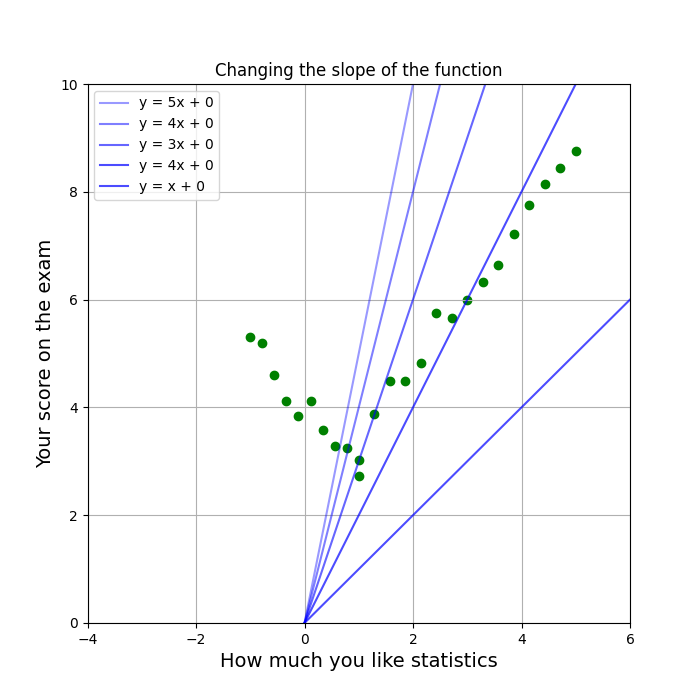
\includegraphics[width=\linewidth]{../images/myplot4.png}
        \caption{Altering the slope parameter of our model}
    \end{minipage}
\end{figure}

We not only tweak the parameter values on their own but also combinations of both of them. To visualize how the loss function depends on parameter values, here is a pretty plot.

\begin{figure}[h]
    \centering
    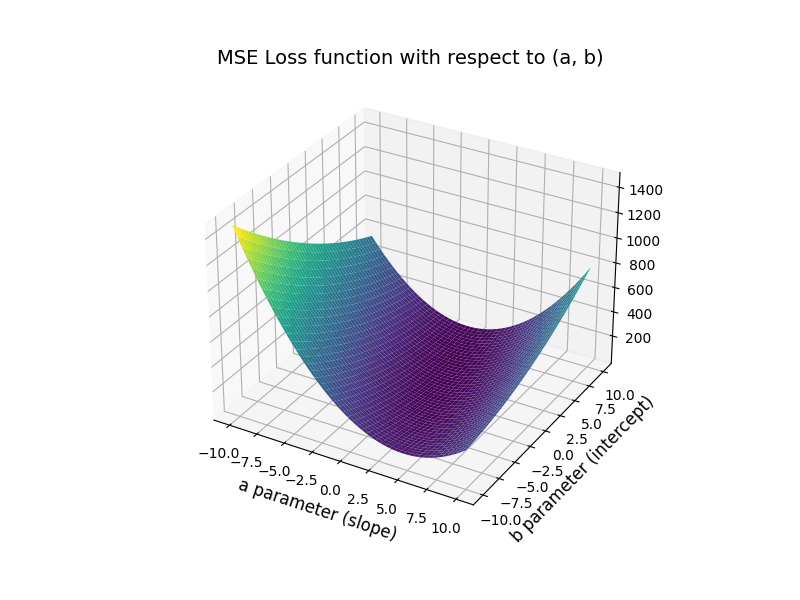
\includegraphics[width=0.66\textwidth]{../images/myplot5.png}
    \caption{Loss with respect to $a$ and $b$}
    \label{fig:loss_3d}
\end{figure}

\break

\section{Random Walking}

Remember how enumeration was structured checking of all possible values? Now with Random Walking, we take the same range of possible values but instead of all combinations, we pick a random number from each domain of possible values for $a$ and $b$ respectfully, and we check the loss at given random point. We do this $N$ times and pick the pair of $(a, b)$ values that results with the smallest loss.

\section{Random Search}

Random Search I believe was explained on the lectures quite well. Basic outline of this algorithm, Starting from a randomly sampled point $p = (a, b)$ we need to define initial range of searching $r$, from the point $p$ we sample another random point in the range $r$, new point is accepted and set as the current point if and only if the loss in new point is smaller.

\begin{figure}[h]
    \centering
    \begin{minipage}{0.4\textwidth}
        \centering
        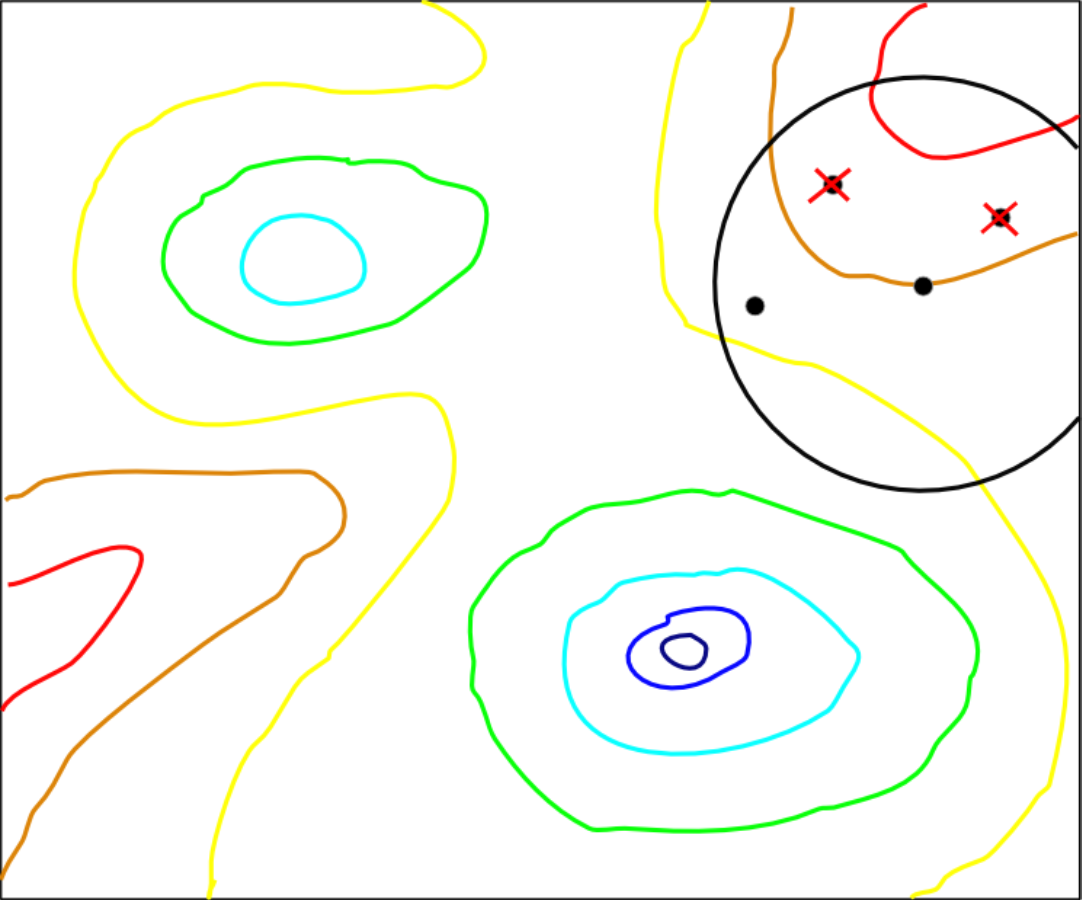
\includegraphics[width=\linewidth]{../images/screenshot1.png}
        \caption{Image from presentation, initial $p$ and few tries of new points.}
    \end{minipage}
    \hfill
    \begin{minipage}{0.4\textwidth}
        \centering
        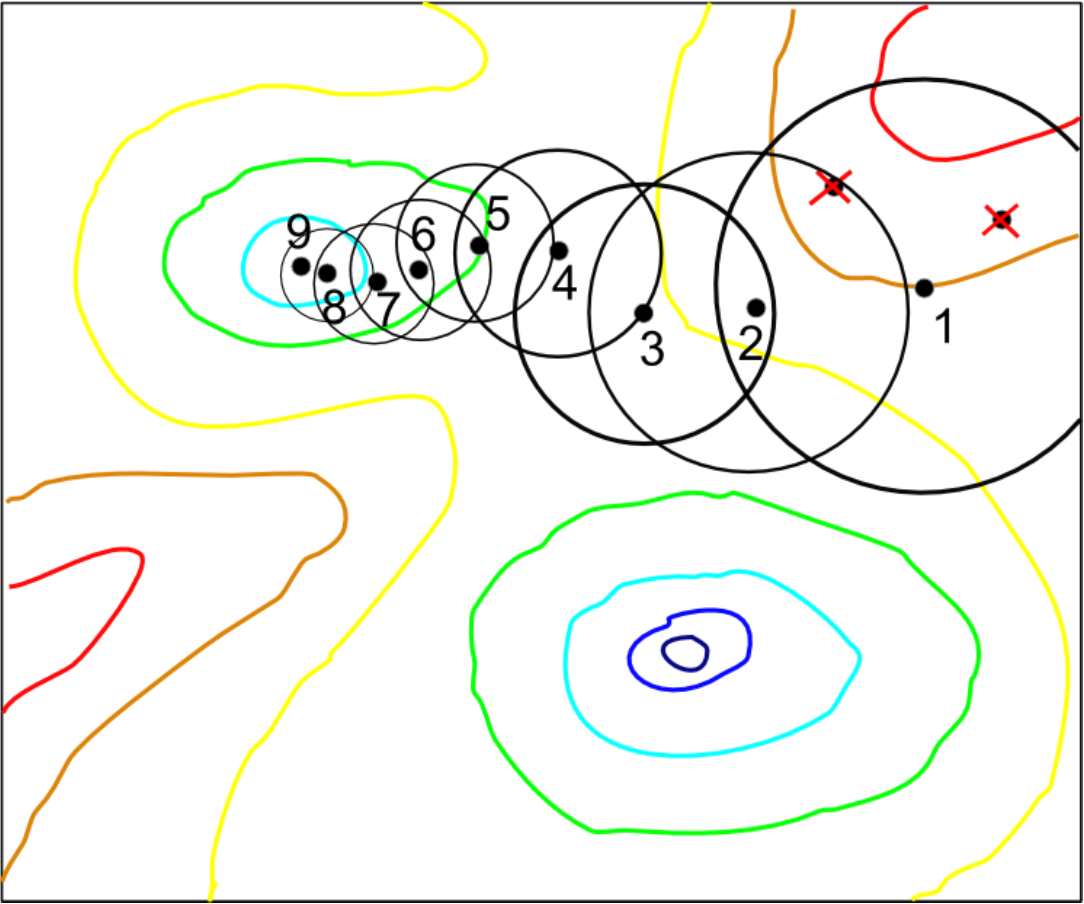
\includegraphics[width=\linewidth]{../images/screenshot2.png}
        \caption{Final state of the algorithm after many points have been sampled, notice how the range of search might be changing.}
    \end{minipage}
\end{figure}

\section{Simulated Annealing}

\section{Gradient Descent/Search}

This is the most commonly used method, especially when it comes to Neural Networks, however it is also the first one that requires us to have knowledge of the exact formula of the loss function. All the previous methods just used sampled values from all possible solutions and corresponding loss. Gradient Descent can be seen as similar to explained above Random Search, in the sense that it is an iterative method, where it differs is the way how the new point is obtained. Using the information about the current value of loss and the formula to obtain it, we can calculate how much and in what direction we should move from current point to obtain a point with lower loss.

\textit{How is it done?} First we need to be able to calculate the Gradient of the function, it is a partial derivative (\textit{Derivative as we lear in high school, just with respect to specified letter}) for all the adjustable components that the loss function depends on, the gradient tells us the direction to nudge each component to increase the loss. \textit{Brace your selfs, the math is coming.}

\begin{align*}
    \mathcal{L}(a,b) &= \frac{1}{N}\sum_{i=1}^N{(y_i - (ax_i + b))^2}\\\\
    \nabla\mathcal{L} &= \left[\frac{\partial \mathcal L}{\partial a}, \frac{\partial \mathcal L}{\partial b}\right]
\end{align*}

\textit{Calm down, don't be scared of fancy symbols} Short explanation: $\nabla$ is just the math symbol for gradient, $\partial$ is a symbol indicating that it is a partial derivative, you might know it's famous brother $d$ for the regular derivative ($\frac{df(x)}{dx}$). Moving on, to calculating the partial derivatives.

\begin{align*}
    \frac{\partial\mathcal L}{\partial a} &= \frac{\partial\mathcal L}{\partial MSE} \frac{\partial MSE}{\partial a} = \frac{\partial\mathcal L}{\partial MSE} \frac{\partial MSE}{\partial R}\frac{\partial R}{\partial a} = \frac{\partial\mathcal L}{\partial MSE} \frac{\partial MSE}{\partial R}\frac{\partial R}{\partial f} \frac{\partial f}{\partial a} \\\\
    MSE(x) &= \frac{1}{N}\sum^N_{i=1}(x_i)^2 \\
    R(y, x) &= y - f(x) \\
    f(x) &= ax + b
\end{align*}

So, lets just say that calculating derivatives is hard, so to simplify we use a chain rule, and when you will be interested you can Google, YouTube, or Chat it. The final partial derivative with respect to $a$.

\begin{equation}
    \frac{\partial\mathcal L}{\partial a} = -\frac{2}{N}\sum_{i=1}^{N}x_i \left(y_i-ax_i-b\right)
\end{equation}

And as the partial derivative with respect to $b$ is similar, here is the formula:

\begin{equation}
    \frac{\partial\mathcal L}{\partial b} = -\frac{2}{N}\sum_{i=1}^{N} y_i - ax_i-b
\end{equation}

\begin{figure}[h]
    \centering
    \begin{minipage}{0.4\textwidth}
        \centering
        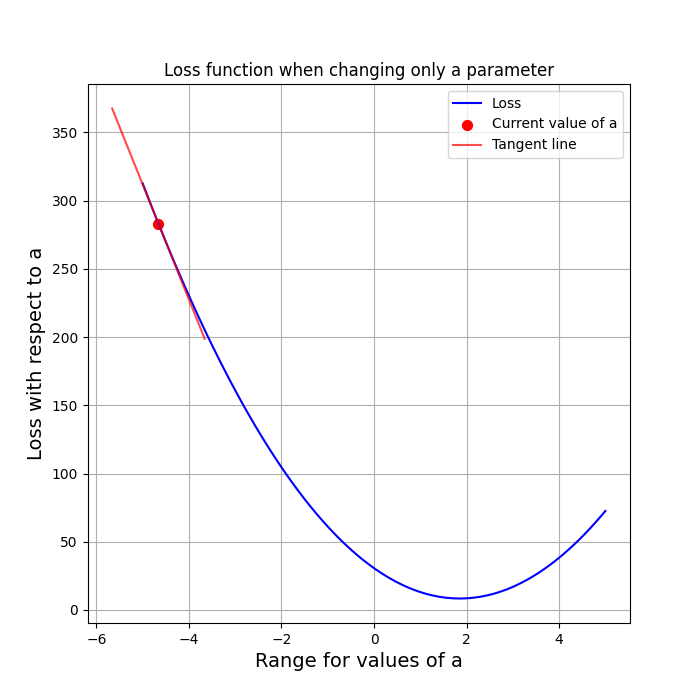
\includegraphics[width=\linewidth]{../images/myplot9.png}
        \caption{Derivative of the Loss with respect to a, visualized as tangent line.}
    \end{minipage}
    \hfill
    \begin{minipage}{0.4\textwidth}
        \centering
        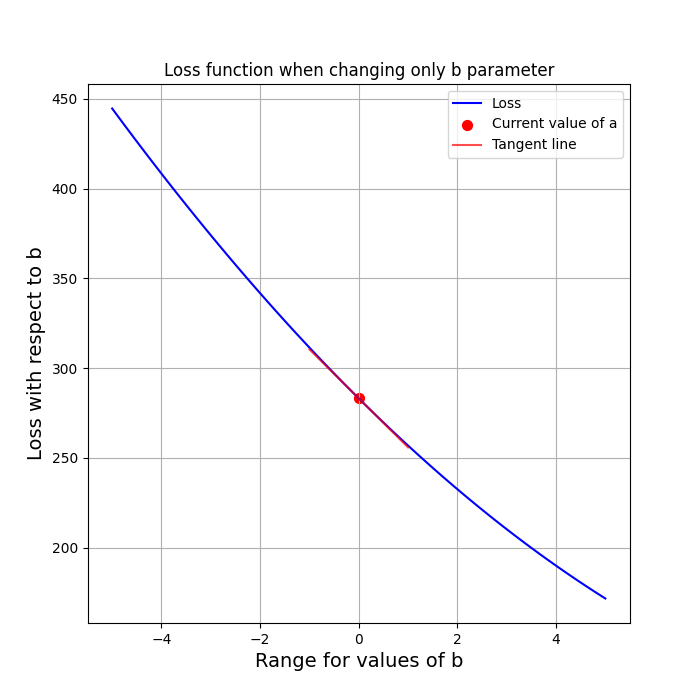
\includegraphics[width=\linewidth]{../images/myplot10.png}
        \caption{Derivative of the Loss with respect to b, visualized as tangent line.}
    \end{minipage}
\end{figure}

With that after plugging in the numbers we get the gradient, so we know in which way to move as the point ti increase the loss, as our task is to minimize the loss we just go in the opposite (negative) direction. Lets again consider $p$ as the current state of our line fitting model. Now to update our model with the gradient we do this:

\begin{equation}
    p_{t+1} = p_t - \eta\nabla\mathcal L
\end{equation}

Where $p_{t+1}$ is some notation to indicate that this is the new/future value if $p_t$, $\nabla\mathcal L$ is our gradient, and $\eta$ is a hyper-parameter called \textbf{Learning Rate} indicating how quickly we want to adjust the weight, typically it is set to something from $\left[0.01, 0.0001\right]$ but generally a very small number, this increases the time necessary for training but makes sure we can find the minimum and not just bounce around it.

In the case of Neural Networks, that operate with loss functions in a lot higher dimensions and a lot less smooth looking, this algorithm can get easily stuck can be hard to train due to the very un even slopes full of local minima, then we could notice gradients that often vary from small to huge. To mitigate this an idea of \textbf{momentum}, also a hyper-parameter, is introduced, it may look terrifying, but the only thing that it does is using part of previous step direction with combination of current step.

\begin{align*}
    \Delta p_t &= \beta \Delta p_{t-1} + (1-\beta)\nabla\mathcal L\\
    p_{t+1} &= p_t - \eta\Delta p_t
\end{align*}

I hope when written like that, it is at least kind of understandable. Moving on, there is one more important and commonly know variant of Gradient Descent, Scholastic Gradient Descent (SGD).

In practice Gradient Descent has a problem, remember the moment when we sum over the Residual of EVERY POINT in out dataset? And as computational power and VRAM are expensive, a SGD comes with a solution. Instead of loading an entire dataset at once we load a single example and calculate the gradient for this single example, this results in a lot less smooth descent, and possibly longer training time, with in the worst case scenario requirements to use scheduling for the learning rate, but on the up side it is less computationally demanding and sometimes leads to better solutions (\textit{Why? The word is not sure, maybe due to it's noisiness it can easier escape narrow local minima.}).

The most commonly used option however is the middle ground, so Batch Processing and SGD, we divide the entire dataset into batches of specific size (ex. 32 data points per batch) we perform the gradient calculations for a single batch and adjust the model weights, then move to the next batch.


\end{document}
